%==============================================================================
% Sjabloon poster bachproef
%==============================================================================
% Gebaseerd op document class `a0poster' door Gerlinde Kettl en Matthias Weiser
% Aangepast voor gebruik aan HOGENT door Jens Buysse en Bert Van Vreckem

\documentclass[a0,portrait]{hogent-poster}

% Info over de opleiding
\course{Bachelorproef}
\studyprogramme{toegepaste informatica}
\academicyear{2025-2026}
\institution{Hogeschool Gent, Valentin Vaerwyckweg 1, 9000 Gent}

% Info over de bachelorproef
\title{Intrusiedetectie in een IoT-omgeving: Evaluatie van Suricata en Zeek op een Single-Board Computer.}
\subtitle{}
\author{Younes Bentaiba Alili}
\email{younes.bentaibaalili@student.hogent.be}
\supervisor{Lieven Smits}
\cosupervisor{Martijn Saelens (Hogeschool Gent)}

% Indien ingevuld, wordt deze informatie toegevoegd aan het einde van de
% abstract. Zet in commentaar als je dit niet wilt.
%\specialisation{Systeem- en Netwerkbeheer}
\keywords{Internet of Things, Intrusion Detection System, Suricata, Zeek, Raspberry Pi}
\projectrepo{https://github.com/ybent/bachelorproef-2026}
\hypersetup{pdfborder={0 0 0}}
\begin{document}

\maketitle

\begin{abstract}
Deze scriptie onderzoekt de geschiktheid van de open-source Intrusion Detection Systems (IDS) Suricata en Zeek op een budgetvriendelijke Single-Board Computer (Raspberry Pi 4) om IoT-verkeer te monitoren. Het onderzoek meet enerzijds structureel het resourcegebruik (CPU en RAM) gedurende verschillende netwerk statussen (rust, normaal verkeer en aanvalstoestanden). Anderzijds richt het onderzoek zich op het ontwikkelen en implementeren van gepaste detectieregels (voor Suricata) en scripts (voor Zeek) om IoT-aanvallen op te sporen.
De resultaten tonen aan dat een Raspberry Pi Krachtig genoeg is voor bedreigingen op te sporen in een klein netwerkomgeving. Beide IDS-systemen kunnen gebruikt worden als een kostenefficiënte beveiligingsoplossing, maar brengen wel een duidelijke architecturale afweging met zich mee. 

\end{abstract}

\begin{multicols}{2} % This is how many columns your poster will be broken into, a portrait poster is generally split into 2 columns
\raggedbottom
\section{Introductie}
IoT-apparaten in kmo's zijn kwetsbaar voor cyberaanvallen, maar commerciële beveiliging is vaak te duur of te complex. Het doel van dit onderzoek is het evalueren en vergelijken van twee open-source Intrusion Detection Systems (IDS) op een single-boardcomputer (zoals een Raspberry Pi) voor het monitoren van IoT-netwerkverkeer.
\section{Methodologie}
Om een realistisch antwoord te krijgen werd er een Proof-of-Concept ontworpen, deze bestond uit vijf fasen:

\begin{enumerate}
    \setlength\itemsep{20pt}
    \item \textbf{Topologie:} Geïsoleerd kmo-netwerk met een MQTT-broker, Zigbee-gateway, fysieke loT-eindpunten en een SPAN-poort (Zie Figuur \ref{fig:topologie}).
    \item \textbf{Implementatie:} Suricata en Zeek onafhankelijk geïnstalleerd op een Raspberry Pi 4.
    \item \textbf{Threat Engineering:} Ontwikkeling van custom signature-regels (Suricata) en event-driven scripts (Zeek).
    \item \textbf{Simulatie:} Uitvoering van actieve netwerkaanvallen.
    \item \textbf{Metingen:} Continue registratie van CPU- en RAM-verbruik tijdens rust (idle), normaal verkeer en aanvallen (stress-test).
\end{enumerate}


\section{Resultaten \& Analyses}
Beide systemen detecteerden succesvol zware netwerkaanvallen zonder de hardwarelimieten van de Raspberry Pi te overschrijden. Dit ging echter gepaard met een duidelijke architecturale \textit{trade-off}:

\begin{itemize}
    \setlength\itemsep{5pt}
    \item \textbf{Suricata (Signature):} Zeer stabiel CPU-verbruik, maar hoog RAM-verbruik bij het inladen van detectieregels.
    \item \textbf{Zeek (Anomaly):} Zeer zuinig met RAM, maar vertoont zware CPU-pieken wanneer scripts actief aanvallen verwerken.
\end{itemize}

\begin{center}
  \captionsetup{type=figure}
  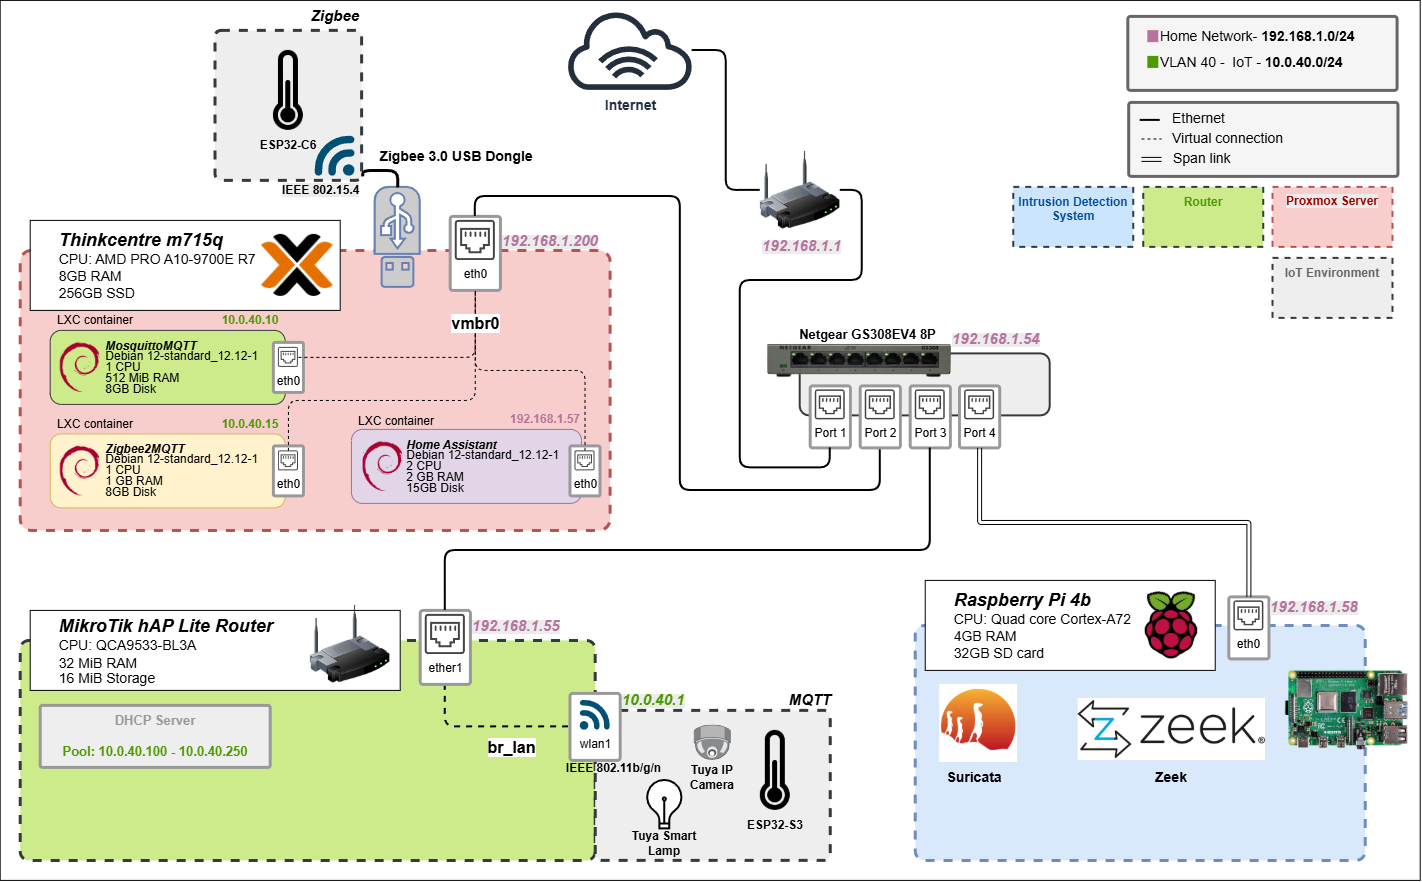
\includegraphics[width=1\linewidth]{../graphics/NetwerkTopologieIoT.png}
  \captionof{figure}{Overzicht van de Proof-of-Concept netwerktopologie, met een geïsoleerd kmo-netwerk en een SPAN-poort op de managed switch voor passieve inspectie.}
  \label{fig:topologie}
\end{center}


\vfill


\begin{center}
  \captionsetup{type=figure}
  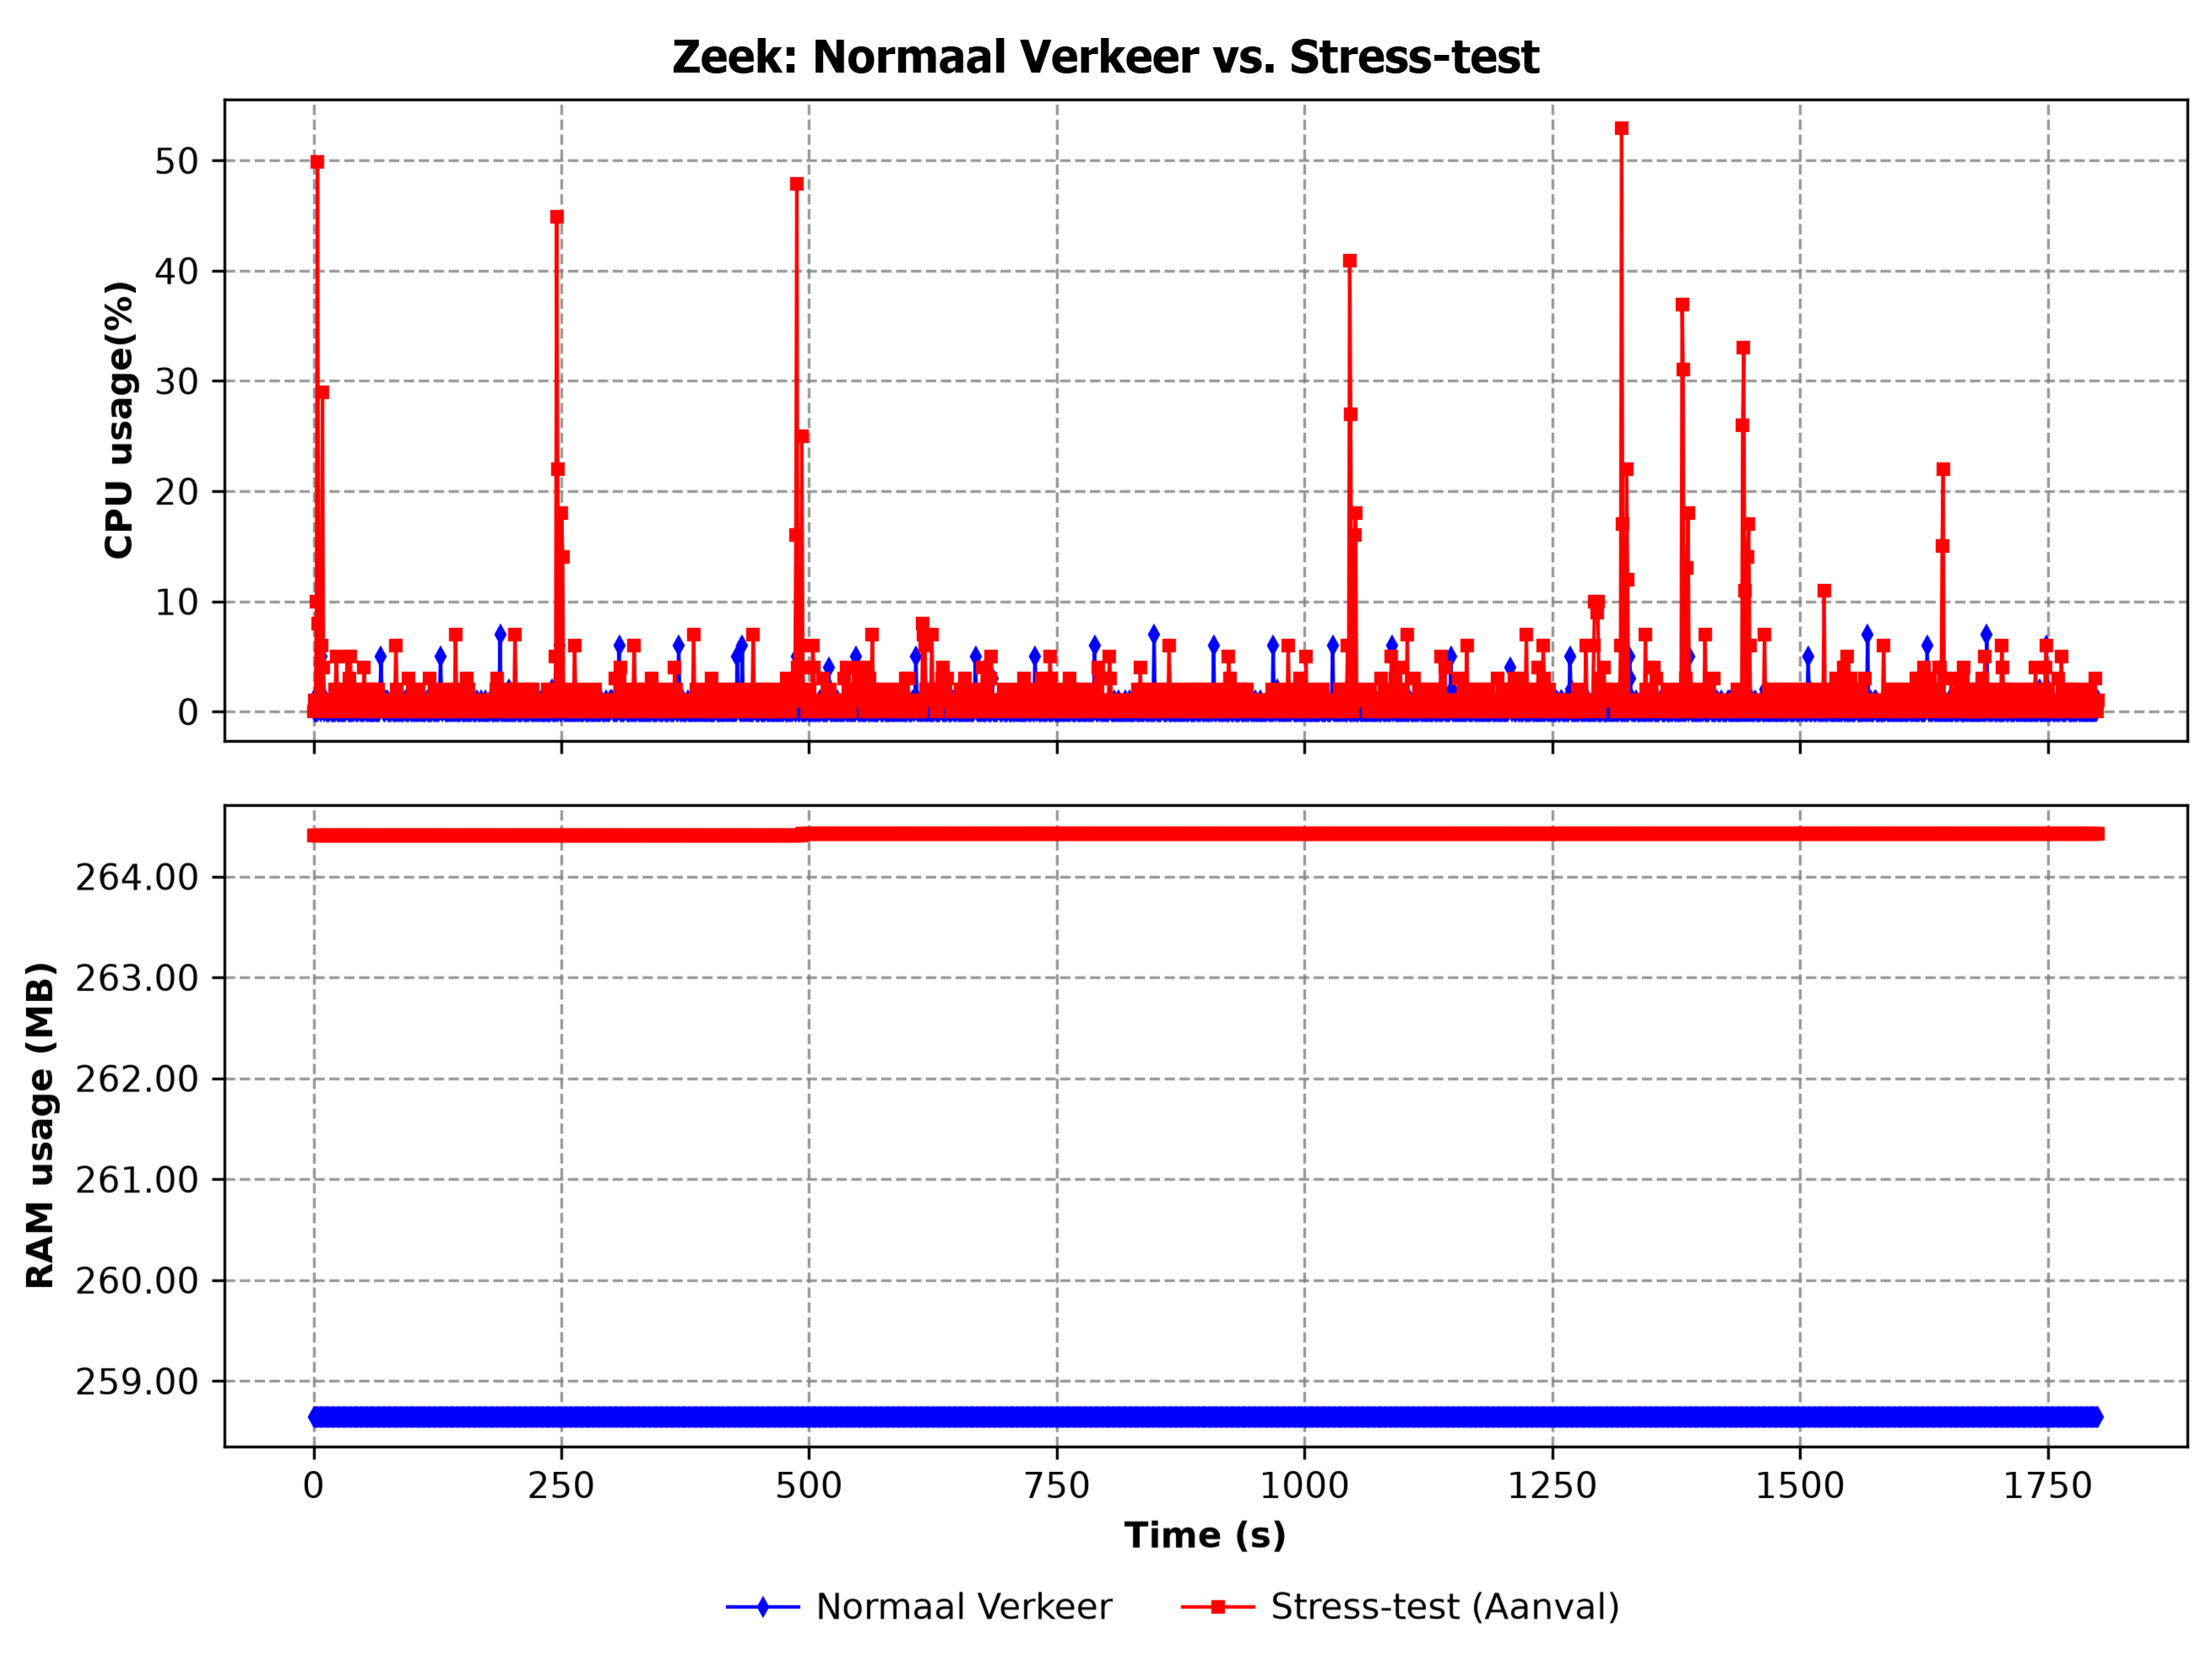
\includegraphics[width=0.8\linewidth]{../graphics/Zeek_poster_plot.png}
  \captionof{figure}{Vergelijking van het CPU- en RAM-verbruik van Zeek tijdens normaal IoT-verkeer versus een actieve netwerkaanval.}
\end{center}

\begin{center}
  \captionsetup{type=figure}
  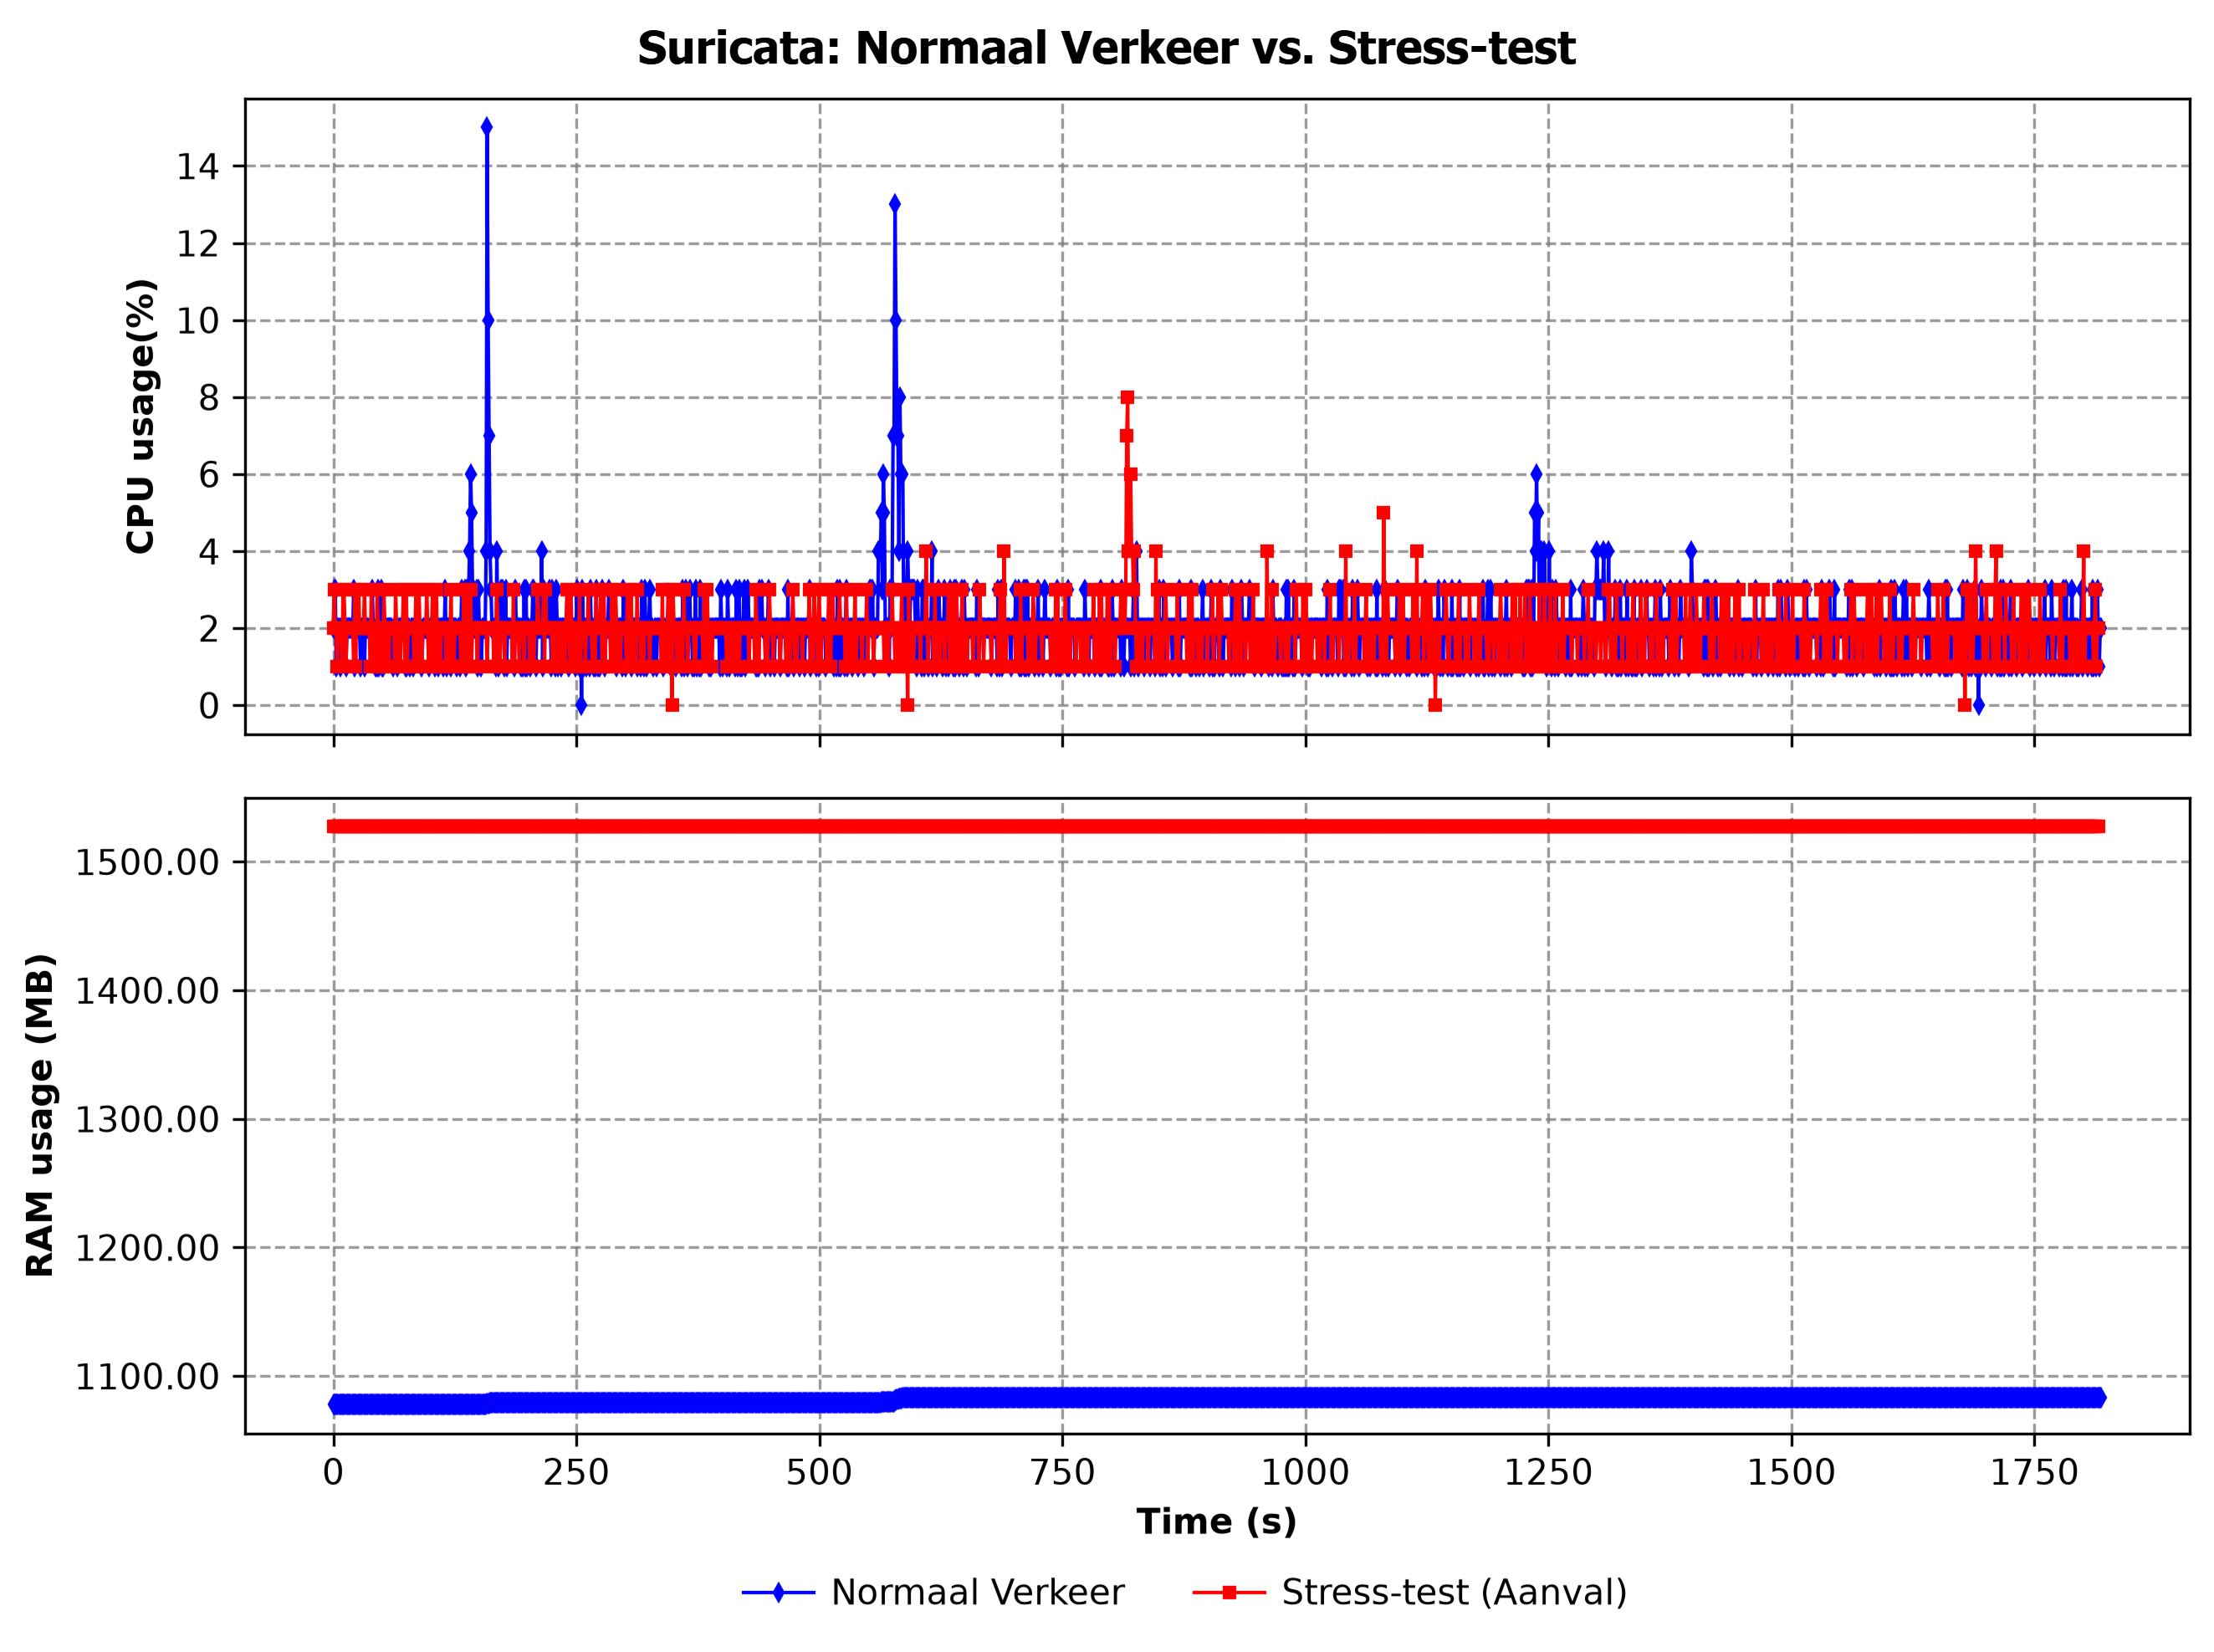
\includegraphics[width=0.8\linewidth]{../graphics/Suricata_poster_plot.png}
  \captionof{figure}{Vergelijking van het CPU- en RAM-verbruik van Suricata tijdens normaal IoT-verkeer versus een actieve netwerkaanval.}
\end{center}


\section{Conclusies}
Dit onderzoek toont aan dat er geen eenduidige, perfecte IDS-oplossing bestaat voor elke kmo, maar bewijst wel dat de aanschaf van dure servers overbodig is. Een budgetvriendelijke Raspberry Pi 4 is krachtig genoeg om zware netwerkaanvallen te detecteren zonder de hardwarelimieten te overschrijden. De beste IDS-keuze hangt direct af van de aanwezige IT-kennis:
\begin{itemize}
    \setlength\itemsep{2pt}
    \item \textbf{Suricata:} Snel en makkelijk in te stellen (\textit{plug-and-play}), maar vereist voldoende RAM.
    \item \textbf{Zeek:} Efficiënt en proactief, maar heeft een steile leercurve door de benodigde scriptkennis.
\end{itemize}

\end{multicols}
\end{document}